% !TeX spellcheck = en_GB
%\documentclass[handout]{beamer}\mode<presentation>{\usetheme{AMSCesenaPurpleAndGold}}
\documentclass[presentation]{beamer}\mode<presentation>{\usetheme{AMSCesenaPurpleAndGold}}
%%%%

\usepackage{sd-lab-ws}
\usepackage{my-listings}
\usepackage{forloop}

\newcommand{\bs}[1]{\textbackslash{}#1}
\newcommand{\labN}{8}
\newcommand{\labGroup}{https://gitlab.com/pika-lab/courses/ds/ay2021}
\newcommand{\labRepo}{\labGroup/lab-\labN}

\title{L\labN{} -- ReSTfull Web Services}
%
\subtitle[SD]{Distributed Systems / Technologies}
%
\author[Ciatto \and Omicini]
{\emph{Giovanni Ciatto} \and Andrea Omicini\\
	\texttt{giovanni.ciatto@unibo.it \and andrea.omicini@unibo.it}}
%
\institute[DISI, Univ. Bologna]
{Dipartimento di Informatica -- Scienza e Ingegneria (DISI)\\\textsc{Alma Mater Studiorum} -- Universit{\`a} di Bologna a Cesena}
%
\date[A.Y. 2020/2021]{Academic Year 2020/2021}

\setbeamercovered{transparent}

\AtBeginSection{
	\begin{frame}[c]\frametitle{Outline}
		% 		\begin{multicols}{2}
		\tableofcontents[sectionstyle=show/shaded, subsectionstyle=hide/hide, subsubsectionstyle=hide/hide]
		% 		\end{multicols}
	\end{frame}
}

\AtBeginSubsection{
	\begin{frame}[c]\frametitle{Next in Line\ldots}
		\begin{multicols}{2}
			\small
			\tableofcontents[sectionstyle=show/shaded, subsectionstyle=show/shaded, subsubsectionstyle=hide/hide]
		\end{multicols}
	\end{frame}
}

\begin{document}
	
%\\\\\\\\\\\\\\\\\\\\\
\frame{\titlepage}
%\\\\\\\\\\\\\\\\\\\\\

\section{Whetting your appetite}

\begin{frame}[allowframebreaks]
\frametitle{Motivation}

\begin{itemize}
    \item \alert{Web services} are a common pattern for nowadays distributed systems
    %
    \begin{itemize}
        \item Probably, most applications you use every day are web services
        \item[eg] Facebook, Instagram, YouTube, PayPal, Spotify, Netflix, and, yaeh, \alert{Trenitalia} too
    \end{itemize}
    
    \vspace{.3cm}

    \item Most web services adhere to the \alert{\emph{Re}presentational \emph{S}tate \emph{T}ransfer} (ReST) architectural style, which is the \emph{de facto} standard for web services
    
    \vspace{.3cm} 

    \item This means they expose a \alert{ReSTfull API} which is used to wrap a server implemented with some arbitrary technology
    %
    \begin{itemize}
        \item Such an API is usually formalised by means of some \alert{specification language} and it is publicly available
        
        \item[eg] \href{https://developers.google.com/apis-explorer/\#p/youtube/v3}{YouTube Data API v3}
    \end{itemize}

    \framebreak

    \item Clients -- possibly implemented with some different technology -- can interact with the web service simply by means of such an API

    \vspace{.3cm}

    \item The ReST principles are often reified into a number of good practices aimed at creating \alert{scalable} and \alert{interoperable} systems which are easy to design, develop, and maintain
    %
    \begin{itemize}
        \item[eg] \url{https://www.restapitutorial.com/}
    \end{itemize}
\end{itemize}
\end{frame}

\begin{frame}%[allowframebreaks]
\frametitle{Lecture Goals}
    \begin{itemize}
        \item Recall the Hyper Text Transfer Protocol (HTTP)
        %
        \begin{itemize}
            \item (Even if it is not the only choice, HTTP is usually the base protocol of choice)
        \end{itemize}
        
        \vfill
        
        \item Understand how ReST principles are reifyied into good practices and patterns for HTTP-based application
        
        \vfill
        
        \item Learn how to produce a (semi-)formal \alert{API specification} by means of de facto standard tools
        
        \vfill
        
        \item Learn how a ReSTful \emph{server} should be designed and implemented
        
        \vfill
        
        \item Learn how pre-existing, local software gave can be \alert{wrapped} within web services and \alert{distributed}
    \end{itemize}
\end{frame}

\section{Recall the HTTP protocol}

\subsection{Overview}

\begin{frame}[allowframebreaks]
\frametitle{HTTP Overview}
    
    \begin{itemize}
        \item One or more \alert{clients} can communicate with a server by means of \alert{synchronous} RPC calls
        
        \vspace{.3cm}
        
        \item Each client issues a \alert{request} and waits for a \alert{response} from the server. In any case:
        %
        \begin{itemize}
            \item requests are directed towards an \alert{URL}, i.e. an name for a resource hosted by the server
            
            \item requests specify a \alert{method}, i.e. an operation with a standard semantics to be performed on the resource
            
            \item responses carry a \alert{status code} with a standard semantics
        \end{itemize}
        
        \vspace{.3cm}
        
        \item Each server is indefinitely \alert{waits} for incoming requests, and, as soon as they arrive, it produces and sends back a response
        %
        \begin{itemize}
            \item in doing, the server may interact with other server or \alert{databases}, behaving as a client w.r.t. them
            
        \end{itemize}
        
        \vspace{.3cm}
        
        \item Requests may possibly provide some \alert{input arguments}, possibly carrying some \alert{return value}
        
        \vspace{.3cm}
        
        \item \alert{Input arguments} may be placed in several places within \alert{Requests}:
        %
        \begin{itemize}
            \item[eg] paths
            \item[eg] query parameters
            \item[eg] headers
            \item[eg] bodies
        \end{itemize}
        
        \vspace{.3cm}
        
        \item \alert{Return values} may be placed in several places within \alert{Responses}:
        %
        \begin{itemize}
            \item[eg] headers
            \item[eg] bodies
        \end{itemize}
    \end{itemize}
    
\end{frame}

\subsection{HTTP Messages Structure}

\begin{frame}{The HTTP \textbf{Request} message structure}
    \centering
    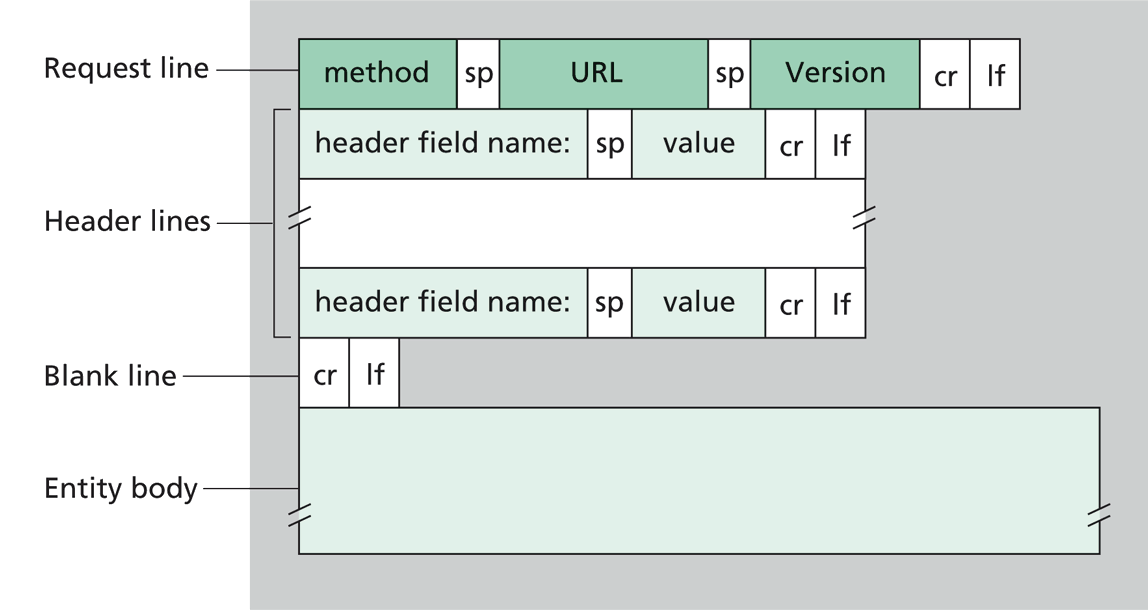
\includegraphics[width=\linewidth]{img/http-req.png}
\end{frame}

\begin{frame}{The HTTP \textbf{Response} message structure}
    \centering
    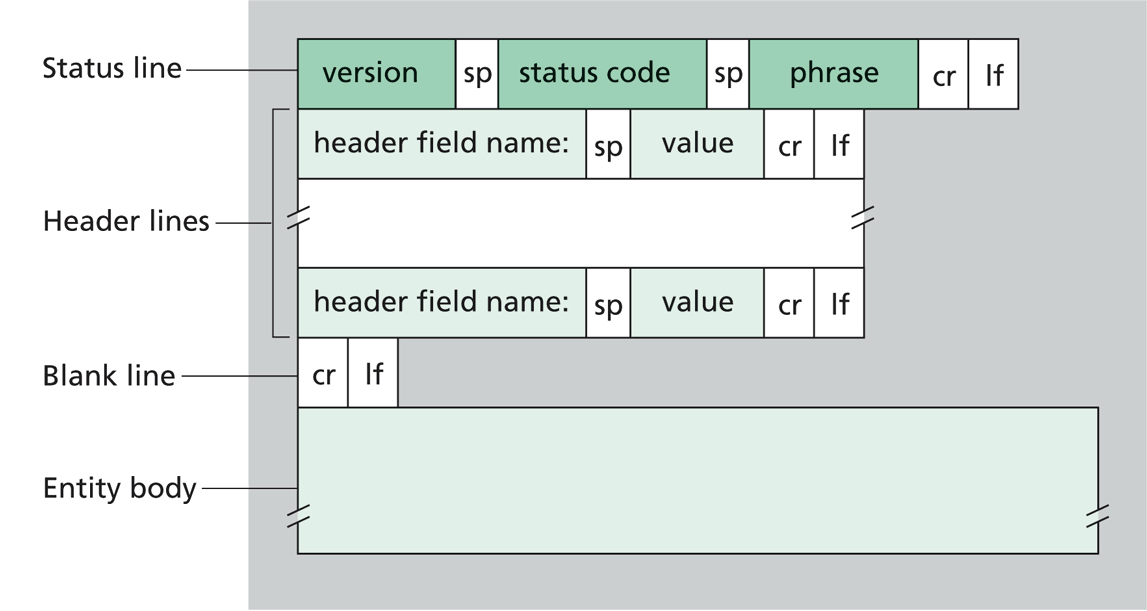
\includegraphics[width=\linewidth]{img/http-res.png}
\end{frame}

\subsection{HTTP Methods}

\begin{frame}{HTTP Methods as CRUD operations}
    \begin{center}
        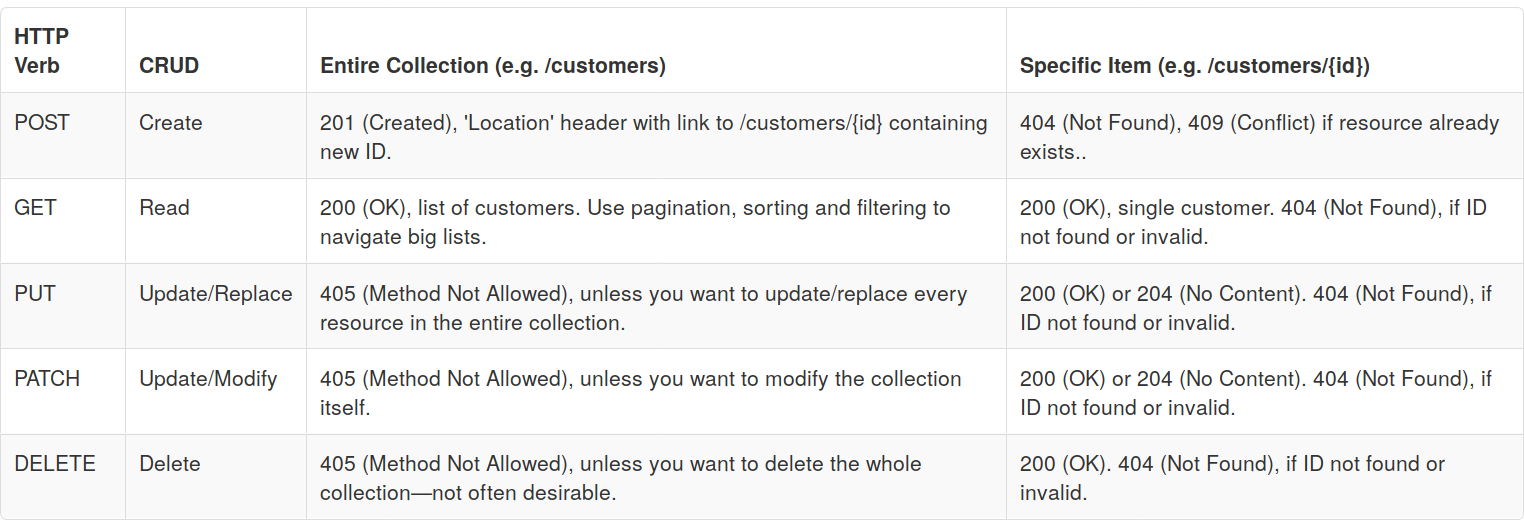
\includegraphics[width=\linewidth]{img/http-methods.png}
    \end{center}
    
    \vfill
    
    \begin{itemize}
        \item CRUD = \emph{C}reate, \emph{R}ead, \emph{U}pdate, \emph{D}elete
        
        \vfill
        
        \item Other HTTP methods exist
        %
        \begin{itemize}
            \item[eg] \texttt{TRACE}, \texttt{HEAD}, \texttt{CONNECT}, or \texttt{OPTIONS}
            \item more details are provided at \url{https://www.w3.org/Protocols/rfc2616/rfc2616-sec9.html}
        \end{itemize}
    \end{itemize}
\end{frame}

\subsection{URL Structure}

\begin{frame}{\textbf{Full} structure of URL}
    \begin{center}
        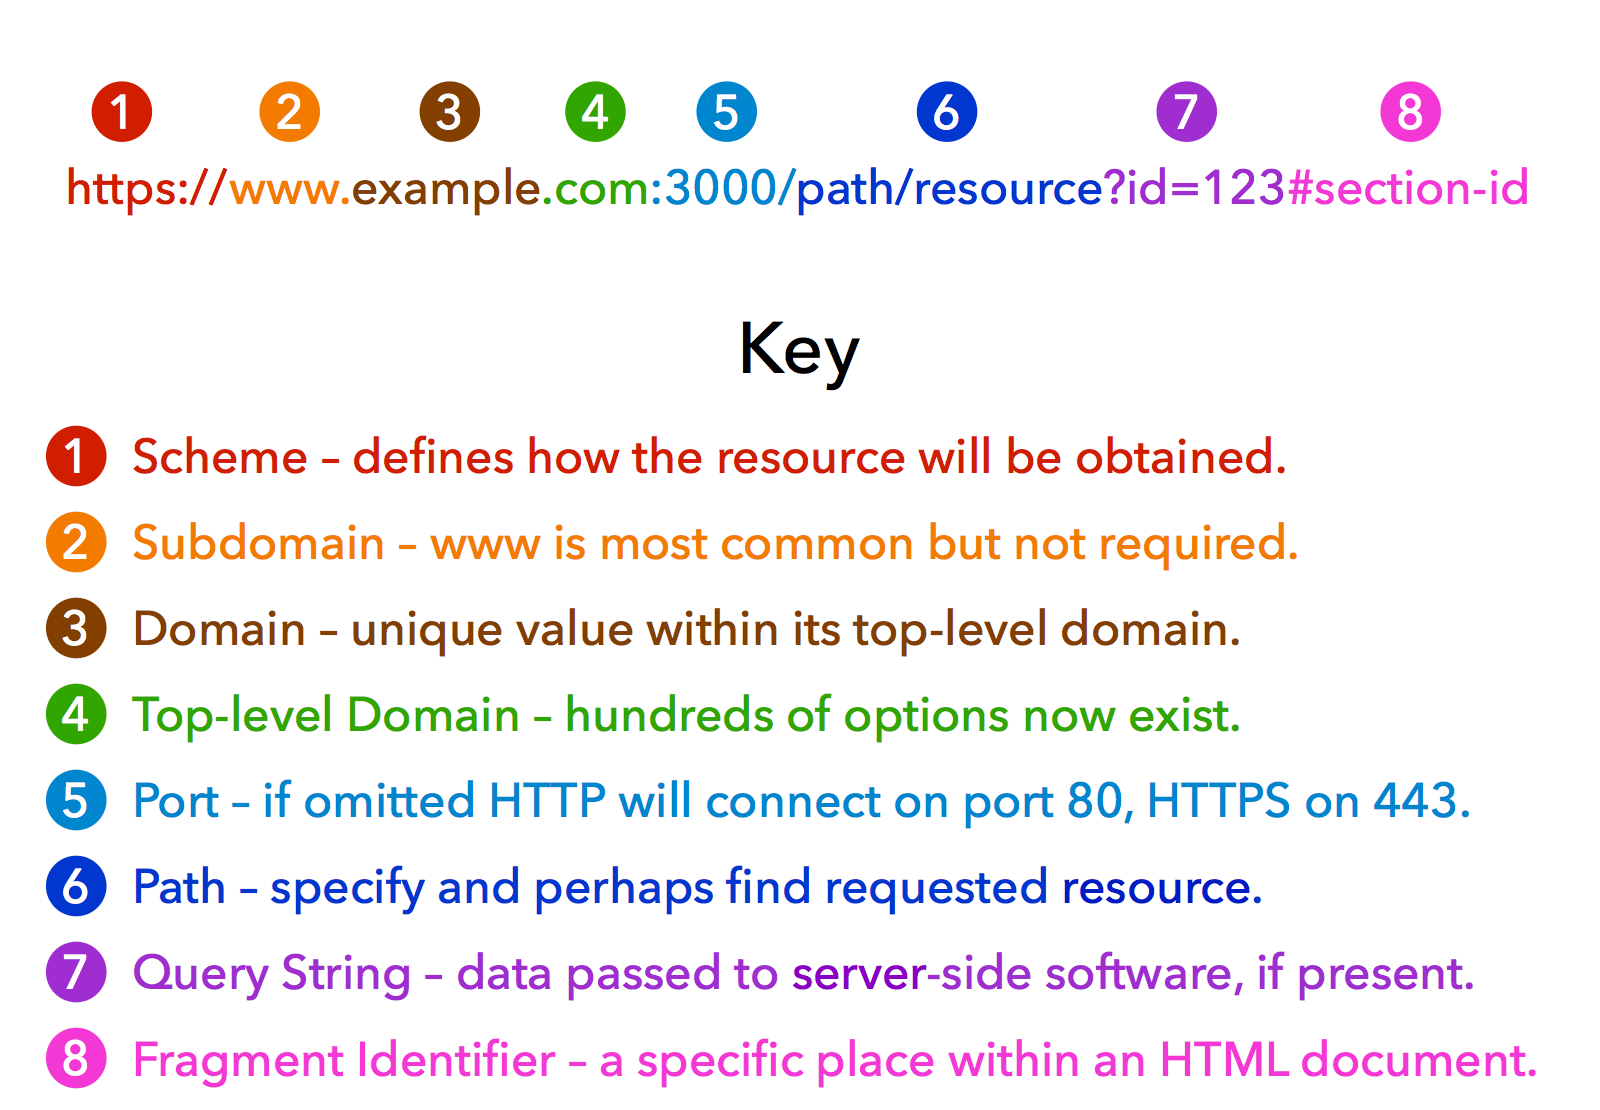
\includegraphics[height=.8\textheight]{img/http-url.png}
    \end{center}
\end{frame}

\begin{frame}{Paths}
    \begin{block}{Paths are usually in the form:}
        \begin{center}
            \texttt{/cathegory/\alert{\{resourceID\}}/subcathegory/\alert{:subResourceID}}
        \end{center}
        %
        where \alert{path parameters} may be denoted through
        %
        \begin{itemize}
            \item curly brackets, e.g. \texttt{\{resourceID\}}
            \item colon, e.g. \texttt{:subResourceID}
        \end{itemize}
    \end{block}

    \begin{exampleblock}{For example, given the parametric URL:}%\small
        \begin{center}
            \texttt{/departments/\alert{\{deptName\}}/professors/\alert{\{profName\}}}
        \end{center}
        one possible instance is:
        \begin{center}
            \texttt{/departments/disi/professors/andrea.omicini}
        \end{center}
        In such case \alert{\texttt{deptName}}=\texttt{disi} and \alert{\texttt{profName}}=\texttt{andrea.omicini}
        
    \end{exampleblock}

\end{frame}

\begin{frame}[allowframebreaks]{Query parameters}
    \begin{block}{Query parameters are \&-separated key-value pairs in the form:}
        \begin{center}
            \texttt{/path/to/resource \emph{?} \alert{key1}=\textit{value1} \emph{\&} \alert{key2}=\textit{value2} \emph{\&} \ldots}
            \\
            {\tiny{}\alert{(without spaces!)}}
        \end{center}
        %
        where
        %
        \begin{itemize}
            \item the \alert{\texttt{'?'}} char denotes the beginning of the query string
            \item the \alert{\texttt{'\&'}} char separates key-value pairs
            \item the \alert{\texttt{'='}} char separates keys from values
        \end{itemize}
    \end{block}
    
    \begin{exampleblock}{For example, the query string:}%\small
        \begin{center}
            \texttt{/students\emph{?}\alert{name}=\textit{Giovanni}\emph{\&}\alert{gender}=\textit{male}}
        \end{center}
        carries two sorts of arguments:
        %
        \begin{description}
            \item[\texttt{name}] whose value is \texttt{Giovanni}
            \item[\texttt{gender}] whose value is \texttt{male}
        \end{description}
        %
        and it is a good way to express the query
        %
        \begin{center}
            \textit{select all male students whose name is ``Giovanni''}
        \end{center}
        %
        according to ReST best practices
        
    \end{exampleblock}
\end{frame}

\begin{frame}{Practical remarks about URLs}
    
    What if some path/query parameter value contains some URL-reserved character like \texttt{'/'}, \texttt{'?'}, \texttt{'\&'}, \texttt{'\#'} or white spaces?
    %
    \begin{itemize}
        \item path/query arguments must be encoded using the \href{https://en.wikipedia.org/wiki/Percent-encoding}{\alert{Percent-encoding}}
        %
        \begin{itemize}
            \item a.k.a. \alert{URL-encoding}
            \item see also \url{https://en.wikipedia.org/wiki/Percent-encoding}
        \end{itemize}
    \end{itemize}
    
    \vfill
    
    \begin{exampleblock}{Example with free text}
    \begin{itemize}
        \item \texttt{Can you read this sentence/phrase?}
        \item \texttt{Can\%20you\%20read\%20this\%20sentence\%2Fphrase\%3F}
    \end{itemize}
    \end{exampleblock}
    
    \vfill
    
    \begin{exampleblock}{Example with regular expression}
    \begin{itemize}
        \item \texttt{\textasciicircum{}message \{ content: (.*?) \}\$}
        \item \texttt{\%5Emessage\%20\%7B\%20content\%3A\%20\%28.\%2A\%3F\%29\%20\%7D\%24}
    \end{itemize}
    \end{exampleblock}
\end{frame}

\subsection{Headers}

\begin{frame}{HTTP Headers}
    \begin{itemize}
        \item HTTP headers allow clients and servers to exchange additional information withing the request or the response, in \alert{piggybacking}
        
        \vfill
        
        \item The general structure of a HTTP header is a colon-separated pairs:
        %
        \begin{center}
        \begin{tabular}{rlc}
            \texttt{StandardHeader\alert{:}} & \texttt{Value} & {\tiny{}(for standard HTTP headers)}
            \\
            \texttt{\alert{X-}CustomHeader\alert{:}} & \texttt{Value} & {\tiny{}(for user-defined headers)}
        \end{tabular}
        \end{center}
        
        \vfill
        
        \item Main headers we will use in this course:
        %
        \begin{description}
            \item[\texttt{Authorization}] | usually present in requests, contains the user credentials, arbitrary encoding
            \item[\texttt{Content-Type}] | usually present in both requests and responses, contains the \alert{MIME-type} of the message body
            \item[\texttt{Accept}] | usually present in requests, contains the \alert{MIME-type(s)} the client is able to understand
        \end{description}
    \end{itemize}
\end{frame}

\subsection{MIME types}

\begin{frame}[allowframebreaks]{MIME types}
    
    \begin{block}{MIME type}
        The \alert{Multipurpose Internet Mail Extensions} (MIME) type is a de-facto standard way to indicate the nature and format of a document
        %
        \begin{itemize}\small
            \item general structure: \alert{\texttt{type/\textit{subType}}}
        \end{itemize}
    \end{block}
    
    \framebreak
    
    \begin{center}
        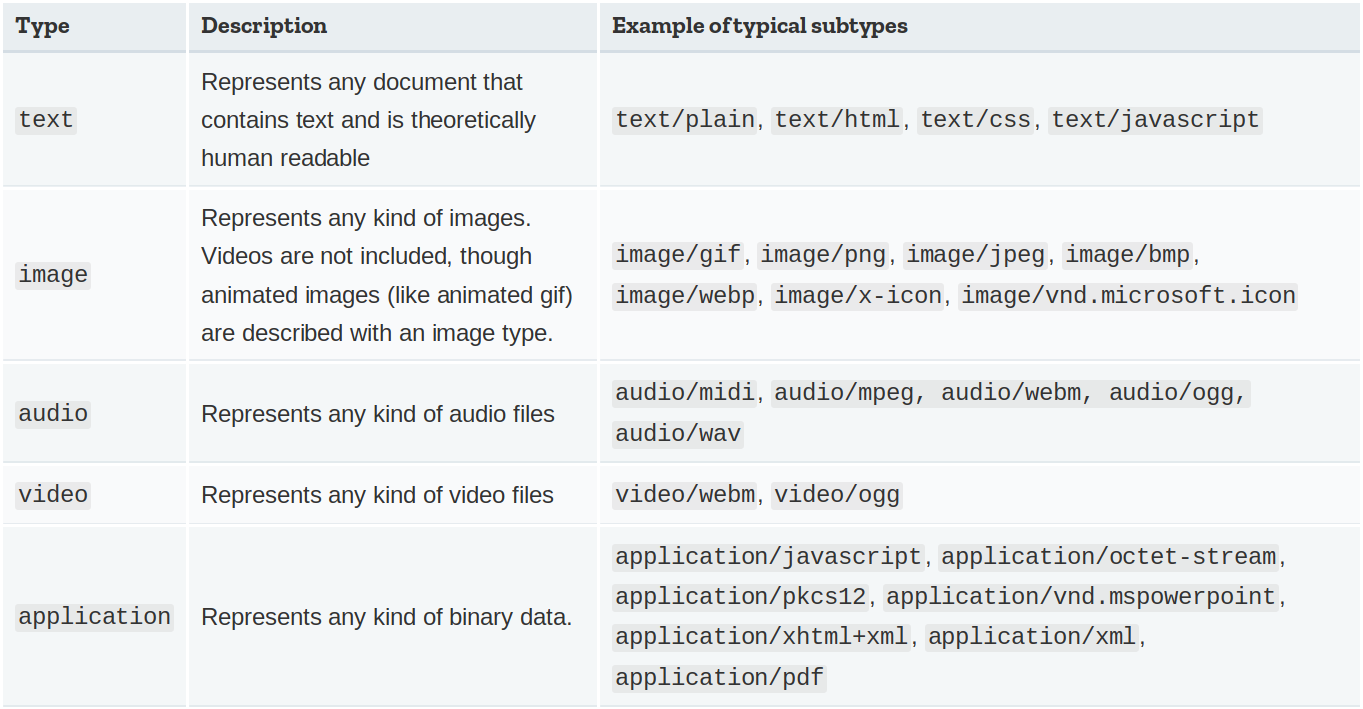
\includegraphics[width=\linewidth]{img/mime_types.png}
        \small
        (Source: \url{https://developer.mozilla.org/en-US/docs/Web/HTTP/Basics_of_HTTP/MIME_types})
    \end{center}
    
\end{frame}

\subsection{Message bodies}

\begin{frame}{Message bodies}
    \begin{itemize}
        \item Message bodies carry the \alert{representations} of the resources being manipulated by the client through the server
        
        \vfill
        
        \item They usually consist of \alert{textual files} adhering to some particular \alert{schema} (i.e. data type)
        
        \vfill
        
        \item Such documents are usually \alert{encoded} according to a MIME type
        %
        \begin{itemize}
            \item Most common ones are \texttt{text/\alert{html}}, \texttt{application/\alert{xml}}, \texttt{application/\alert{json}}, and \href{https://en.wikipedia.org/wiki/YAML}{\texttt{application/\alert{yaml}}}
        \end{itemize}
        
        \vfill
        
        \item Schemas are usually defined by means of \alert{schema languages}:
        %
        \begin{itemize}
            \item \href{https://www.w3schools.com/xml/schema_intro.asp}{XML Schema} for XML
            
            \item \href{https://json-schema.org/learn/getting-started-step-by-step.html}{JSON Schema} for JSON or YAML
            
            \item Some attempts exist to create a (more) target-neutral schema language: \href{https://swagger.io/specification/\#schemaObject}{Open API specification}
        \end{itemize}
    \end{itemize}
\end{frame}


\begin{frame}{Example -- OpenAPI schema for \texttt{User} data type}
    \vspace{-.7cm}
    \begin{columns}[t]
        \begin{column}{.49\textwidth}
            \lstinputlisting[language=yaml]{code/User.yaml}
        \end{column}
        \hfill
        \begin{column}{.49\textwidth}
            \lstinputlisting[language=yaml]{code/UserInstance.yaml}
            \lstinputlisting[language=yaml]{code/UserInstance.json}
        \end{column}
    \end{columns}
\end{frame}

\subsection{Status Codes}

\begin{frame}{HTTP Status Codes -- Overview}
    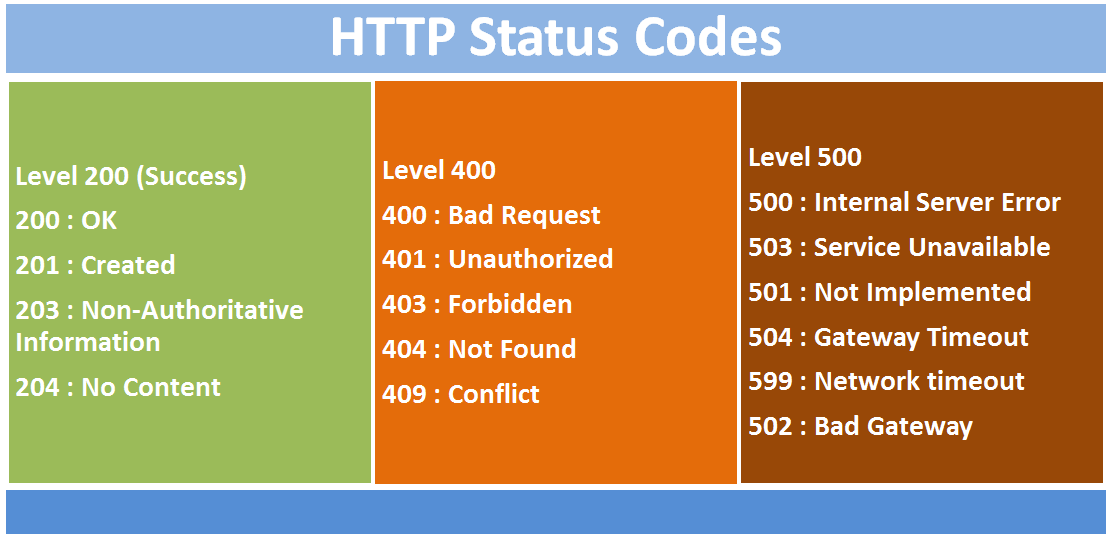
\includegraphics[width=\linewidth]{img/http_status_codes.png}
\end{frame}

\begin{frame}[allowframebreaks]{HTTP Status Codes -- Ranges}
    \begin{block}{\texttt{1xx} -- Informational}
        \begin{center}
            The request was received, continuing process
        \end{center}
    \end{block}
    
    \begin{block}{\texttt{2xx} -- Success}
        \begin{center}
            The request was successfully received, and accepted
        \end{center}
        %
        \begin{itemize}
            \item[eg] \alert{\texttt{200 OK}}: Standard response for successful HTTP requests
            
            \item[eg] \alert{\texttt{204 No Content}}: Like 200 but response contains \alert{no body}
        \end{itemize}
    \end{block}
    
    \begin{block}{\texttt{3xx} -- Redirection}
        \begin{center}
            Further action are needed to complete the request
        \end{center}
    \end{block}
    
    \begin{block}{\texttt{4xx} -- Client Error}
        \begin{center}
            The request contains bad syntax or cannot be fulfilled
        \end{center}
        %
        \begin{itemize}
            \item[eg] \alert{\texttt{400 Bad Request}}: The server cannot or will not process the request due to an apparent client error (e.g., malformed request syntax)
            
            \item[eg] \alert{\texttt{401 Unauthorized}}: Authentication is required and has failed or has not yet been provided
            
            \item[eg] \alert{\texttt{403 Forbidden}}: Authentication was successful but the client has no permission to perform the requested operation
            
            \item[eg] \alert{\texttt{409 Conflict}}: Indicates that the request could not be processed because of conflict in the current state of the resource
        \end{itemize}
    \end{block}
    
    \begin{block}{\texttt{5xx} -- Server Error}
        The server failed to fulfill an apparently valid request
        %
        \begin{itemize}
            \item[eg] \alert{\texttt{500 Internal Server Error}}: A generic error message
            
            \item[eg] \alert{\texttt{501 Not Implemented}}: The server either does not recognize the request method, or it lacks the ability to fulfil the request
        \end{itemize}
    \end{block}
\end{frame}

\subsection{Routes}

\begin{frame}{Routes}
    
    \begin{itemize}
        \item The behaviour of WS is designed \& implemented through \alert{routes}
        
        \vfill
        
        \item There is no precise definition of what a route is, however the expression roughly refers to some \alert{possible operation} the service may expose to let clients manipulate some \alert{resource}
        %
        \begin{itemize}
            \item[eg] think about a method signature in some Java interface
        \end{itemize}
        
        \vfill
        
        \item ``Route'' is usually a \alert{jargon} for:
        %
        \begin{itemize}
            \item[+] an HTTP \alert{method}
            
            \item[+] a (possibly \emph{parametric}) URL
            
            \item[+] a set of input arguments, along with their schema, place (URL, body, query, header), and supported encoding
            
            \item[+] a set of possible status codes, along with their result types \& encoding
        \end{itemize}
        
        \vfill
        
        \item The service \alert{Web API} consists of the set of its routes declarations
        
        \vfill
        
        \item Example of \alert{Web API} \url{https://petstore.swagger.io}
    \end{itemize}
    
\end{frame}

\section{ReSTfull WS Design}

\subsection{Workflow}

\begin{frame}{ReST project design workflow}

When designing a ReST-full web-service, you are encouraged to follow this procedure:
%
\begin{enumerate}
    \item structure your application in terms of \alert{resources} and \alert{sub-resources}
    
    \vfill
    
    \item for each (sub-)resource, define a possibly parametric \alert{path}
    
    \vfill
    
    \item for each path, define the \alert{methods} it supports, thus defining a \alert{route} 
    
    \vfill
    
    \item for each route, define:
    %
    \begin{enumerate}
        \item the supported \alert{query parameters} for the request
        
        \item the supported input \alert{MIME types} and the \alert{schema} of the request body. if any
        
        \item all the possible results, i.e.:
        %
        \begin{itemize}
            \item all possible \alert{status codes}\ldots
            
            \item \ldots and the corresponding schemas for the response bodies
            
        \end{itemize}
        
        \item optionally, you may also define if \alert{authentication} is required and which sorts of \alert{authorizations} are needed
    \end{enumerate}
\end{enumerate}

\end{frame}

\subsection{OpenAPI Specification}

\begin{frame}{OpenAPI Specification and Swagger}

The design and test phases of a ReST-full web service \alert{API} can be greatly simplified by some (almost) standard technologies:
%
\begin{itemize}
    \item The \alert{OpenAPI Specification} (OAS) is a formal language for describing the API of the service
    %
    \begin{itemize}
        \item Current version of the specification is \href{https://github.com/OAI/OpenAPI-Specification/blob/master/versions/3.0.2.md}{version 3.0.2}, but we will use \href{https://github.com/OAI/OpenAPI-Specification/blob/master/versions/2.0.md}{version 2.0} since it is more mature
    \end{itemize}
    
    \vfill
    
    \item In practice, one may actually define a service API by writing a \alert{YAML/JSON file} adhering to the OAS
    
    \vfill
    
    \item \href{https://swagger.io}{Swagger} is a community developing and maintaining the OAS, other than a number of useful tools easing the life of API designers and implementors
    %
    \begin{itemize}
        \item \href{https://editor.swagger.io}{Swagger Editor} is a web-based editor for writing specification files
        
        \item \href{https://swagger.io/tools/swagger-codegen/}{Swagger Codegen} is a tool generating client and server stubs out of an OAS specification file
        
        \item \href{https://app.swaggerhub.com}{SwaggerHub} is a web repository letting people edit, store, and publish their services APIs
    \end{itemize}

\end{itemize}

\end{frame}

\begin{frame}[allowframebreaks]{Main structure of a OAS specification file}
    \lstinputlisting[language=yaml]{code/SwaggerMain.yaml}
\end{frame}

\begin{frame}[allowframebreaks]{Route definition example}
    \lstinputlisting[language=yaml]{code/RouteExample.yaml}
\end{frame}

%===============================================================================
\section*{}
%===============================================================================

%\\\\\\\\\\\\\\\\\\\\\
\frame{\titlepage}
%\\\\\\\\\\\\\\\\\\\\\

%%===============================================================================
%\section*{\refname}
%%===============================================================================
%
%%\\\\\\\\\\\\\\\\\\\\\
%%%%%
%%\begin{frame}[t,allowframebreaks]\scriptsize
%\begin{frame}[c]\footnotesize
%\frametitle{\refname}
%\bibliographystyle{apalike}
%\bibliography{sd-lab-jadelike-agents}
%\end{frame}
%%\\\\\\\\\\\\\\\\\\\\\

%%%%%%%%%%%%%%%%%%%%%%%%%%%%%%%%%%%%%%%%%%%%%%%%%%%%%%%%%%%%%%%%%%%%%%%%%%%%%%%
\end{document}
%%%%%%%%%%%%%%%%%%%%%%%%%%%%%%%%%%%%%%%%%%%%%%%%%%%%%%%%%%%%%%%%%%%%%%%%%%%%%%%%

